\documentclass[8pt, landscape, fleqn]{scrartcl}
\setlength{\parindent}{0pt}
\usepackage[ngerman]{babel}
\usepackage[applemac]{inputenc}
\usepackage[dvips]{geometry}
\usepackage{latexsym}
\usepackage{multicol}
\usepackage{amsmath}
\usepackage{graphicx}
\usepackage{array}
\usepackage{booktabs}
\usepackage{amsmath}
\usepackage{mathtools}
\usepackage{ulem}
\usepackage{amsfonts}
\usepackage{dsfont}
\usepackage{charter} %%% Schreibart
%\renewcommand{\familydefault}{\sfdefault}



%%%%%%%%%%Paket für Chemische Formeln
\usepackage{chemformula} 
\usepackage[version=3]{mhchem}
%%%%%%%%%%%%%%%%% Farbe
\usepackage{color}

\pagestyle{plain}
\typearea{20}
\columnsep 30pt
\columnseprule .4pt
\setlength{\extrarowheight}{0.9em}

\renewcommand{\arraystretch}{0.8}

\makeatletter
\renewcommand{\section}{\@startsection{section}{1}{0mm}%
{-2\baselineskip}{0.8\baselineskip}%
{\hrule depth 0.2pt width\columnwidth\hrule depth1.5pt
width0.25\columnwidth\vspace*{1.2em}\Large\bfseries\rmfamily}}
\makeatother


\makeatletter
\renewcommand{\subsection}{\@startsection{subsection}{1}{0mm}%
{-2\baselineskip}{0.8\baselineskip}%
{\hrule depth 0.2pt width\columnwidth\hrule depth0.75pt
width0.25\columnwidth\vspace*{1.2em}\large\bfseries\rmfamily}}
\makeatother

\makeatletter
\renewcommand{\subsubsection}{\@startsection{subsubsection}{1}{0mm}%
{-2\baselineskip}{0.8\baselineskip}%
{\hrule depth 0.2pt width\columnwidth\vspace*{1.2em}\normalsize\bfseries\rmfamily}}
\makeatother

\newcommand{\Mx}[1]{\begin{bmatrix}#1\end{bmatrix}}
\begin{document}
\part*{\LARGE\textrm{Thermodynamik II - LAV $\hfill$ Xeno Meienberg}}
\begin{multicols*}{3}

\section*{Konstanten}
\begin{itemize}
\item Normdruck: $p_{ref} = 1 atm = 1.01325 \: bar$
\item Normtemperatur: $T_{ref} = 298 \: K \approx 25^{\circ} \: C$
\item Pferdest"arke:  $ 1 \: hp = 1 \: PS = 0.735 \: kW$
\item Elementarladung:  $e=1.60219 \cdot 10^{-19} \:C$
\item Faraday-Konstante: $F= N_A \cdot e = 96485.3 \frac{C}{mol} = \frac{A\cdot s}{mol}$
\item ppm = parts per million: $1 \: ppm = 10^{-6}$
\item Gaskonstante: $ \overline{R} = 8.314 \frac{J}{mol K}$, spez. -- $R = \frac{\overline{R}}{M} [\frac{J}{kg K}]$
\end{itemize}


\section*{Gr"ossen}
\begin{itemize}
\item Molar $ \leftrightarrow $ Massenspezifisch: $n=\frac{m}{M}$
\item Molanteil (Volumenanteil): $\chi_i =\frac{n_i}{ \Sigma_{i} n_i}= \frac{n_i}{n_{net}} = \frac{V_i}{\Sigma V_i} =\frac{V_i}{V_{net}}$
\item Partialdruck: $p_i = \chi_i \cdot p_{net} = \chi_i \cdot p_{tot} $
\item Konzentration (molar): $c_i = n_i / V_{net} $
\item Massenanteil: $Y_i = \frac{m_i}{m_{net}} = X_i \cdot M_i \cdot \frac{\Sigma_j n_j}{\Sigma_j n_j \cdot M_j}$
\item Luft"uberschussfaktor: $\lambda = \frac{(m_L / m_B)}{(m_L / m_B)_{st"och}} = \frac{(\dot{m}_L / \dot{m}_B)}{(\dot{m}_L / \dot{m}_B)_{st"och}} = \frac{(n_L/n_B)}{(n_L/n_B)_{st"och}}$
\item Isentropenkoeffizient: $\kappa = \frac{c_p}{c_v} = \frac{c_v+R}{c_v}= 1 + \frac{R}{c_v} = \frac{c_p}{c_p-R}$
\item $\frac{m_L}{m_{B}} = \frac{M_{O2} + 3.76M_{N_2}}{M_B} \cdot \frac{n_L}{n_B}$
\item Rauchgas $\longrightarrow$ Summe aller Massen der Produkte $\longrightarrow$ Dreisatz $\longrightarrow$1kg Rauchgas entspricht $\longrightarrow$ So und soviel Mol der einzelnen Produkte
\end{itemize}


\section*{Chemische Reaktionen}
\subsection*{St"ochiometrie}
\begin{enumerate}
\item Atome z"ahlen
\item Zuerst diejenigen, die in wenigen Produkten vorkommen
\item Alle Atome des Eduktes ausgleichen
\item Sauerstoff ausgleichen
\item Koeffizient f"ur den inerten Stickstoff "ubernehmen
\end{enumerate}
{\bf{Wichtig: st"ochiometrische Verbrennung = kein unverbrannter Sauerstoff $\Leftrightarrow \lambda = 1$}}
\subsubsection*{Beispiel}
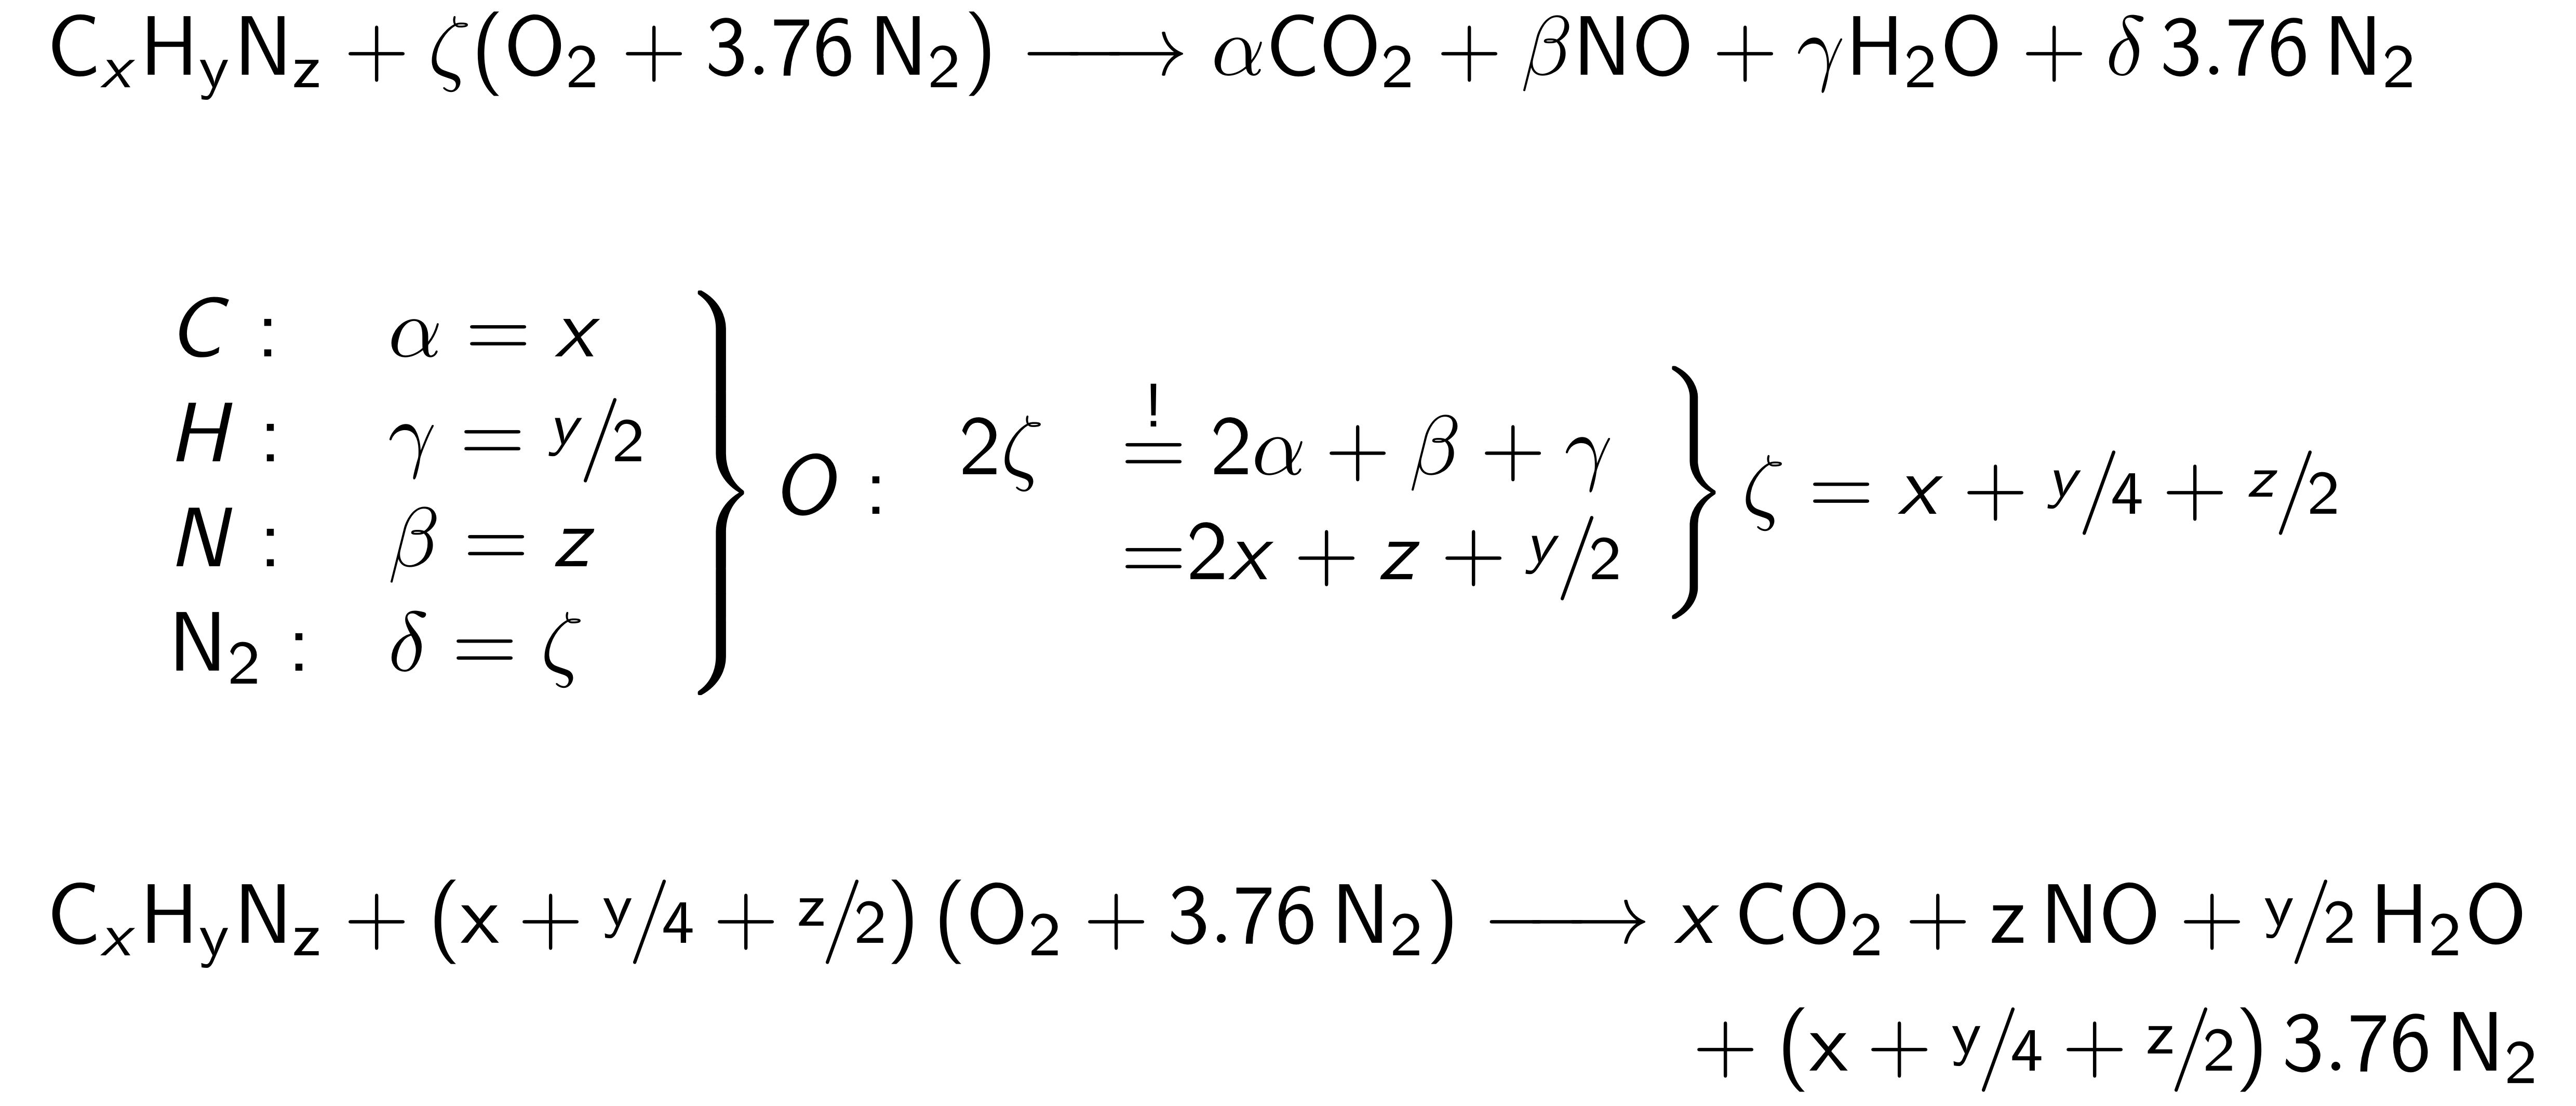
\includegraphics[width=8cm]{Bild01_Summary1_THDII}

\subsection*{Enthalpie einer Substanz}
\begin{equation}
h = h_{f}^{0} + [h(T) - h(T_{ref})]
\end{equation}
{\bf{Standardbildungsenthalpie}} $h_{f}^{0}$ (Tab. A-30):
\begin{itemize}
\item Stoffeigenschaft
\item Wieviel Energie steckt im Molek"ul ? (Bindungen, Wechselwirkungen etc.)
\item Molek"ule im stabilen Zustand (\ce{O2},\ce{N2}, \ce{H2}) haben $h_{f}^{0} = 0$
\end{itemize}
{\bf{Enthalpiedifferenz}} zum Referenzzustand (Tab A-23 bis A-28)
\begin{itemize}
\item Temperaturabh"angig, Annahme: ideale Gase
\end{itemize} 

\subsection*{Reaktionsw"arme $Q_R$ - $\Delta H_R$}
{\bf{Die Reaktionsw"arme $Q_R$ ist die Differenz der (Bildungs)entahlpien $\Delta H_R$! Sie entspricht der Enthalpiedifferenz, wenn Produkte und Edukte bei gleichen Bedingungen vorliegen. Hier rechnen wir immer in Abh"angigkeit des Brennstoffs in kg bzw. in mol. ($Q_R =$ abgegebene W"arme)}}
\begin{itemize}
\item Unter Standardbedingungen: \[-Q_R = \Delta H_R = \sum_{Produkte} \nu''_j h_{f}^{0} - \sum_{Edukte} \nu'_j h_{f}^{0} \quad  \Big[\frac{kJ}{kg} \Big] \]
\item Bei anderer Temperatur ($T_{Edukte}=T_{Produkte}$): \[= \sum_{Produkte} \nu''_j (h_{f}^{0} + h(T) - h(T_{ref})) -\sum_{Edukte} \nu'_j (h_{f}^{0} + h(T) - h(T_{ref})) \]
\end{itemize}


\subsubsection*{Verbrennung von Ammoniak - ohne Luft"uberschuss}
\ce{NH3 + 5/4 (O2 + 3.76 N2) -> NO + 3/2 H2O + 5/4 (3.76 N2)}
\subsubsection*{Verbrennung von Ammoniak - mit Luft"uberschuss}
\ce{NH3 + 5/4 \lambda (O2 + 3.76 N2) -> NO + 3/2 H2O + 5/4 (\lambda-1) O2 + 5/4 \lambda (3.76 N2)} \\


Hier taucht der "ubersch"ussige, unverbrannte Sauerstoff $(\lambda-1)$ nochmals auf. Falls zu wenig Luft vorhanden ist dementsprechend $(1-\lambda)$ Sauerstoff vorhanden



\subsection*{Verbrennung von Kohlewasserstoffen}
F"ur $\lambda \geq 1$ (mager, st"ochiometrisch):
\begin{itemize}
\item \ce{C_xH_y + \lambda (x + $\frac{y}{4}$) (O2 + 3.76 N2) -> x CO2 + $\frac{y}{2}$ H2O + ( \lambda -1 ) ( x +$\frac{y}{4}$) O2 + \lambda $\cdot$ 3.76 (x + $\frac{y}{4}$) N2 }
\end{itemize}
F"ur $\lambda < 1$ (fett): 
\begin{itemize}
\item \ce{C_xH_y + \lambda (x + $\frac{y}{4}$) ( O2 + 3.76 N2 ) -> (1 -\lambda) C_xH_y + \lambda x CO2 + $\frac{\lambda y}{2}$ H2O + 3.76 \lambda (x +$\frac{y}{4}$) N2 }
\end{itemize}


\subsection*{Verbrennung von Alkoholen}
F"ur $\lambda \geq 1$:
\begin{itemize}
\item \ce{C_xH_yO_z + \lambda (x + $\frac{y}{4}$ - $\frac{z}{2}$) ( O2 + 3.76 N2 ) -> x CO2 + $\frac{y}{2}$H2O + (\lambda  -1) (x + $\frac{y}{4}$ -$\frac{z}{2}$) O2 + 3.76 \lambda (x + $\frac{y}{4}$ -$\frac{z}{2}$) N2   }
\end{itemize}
Bei $\lambda < 1$ verbleiben in den Produkten Anteile des Brennstoffs $\rightarrow$ unverbrannte Kohlenwasserstoffe

\subsection*{Adiabate Flammtemperatur}
Diejenige Temperatur, die erreicht wird, wenn der Reaktor\slash Brennkammer adiabat ist und keine Arbeit leistet (maximale, theoretische Prozesstemperatur)
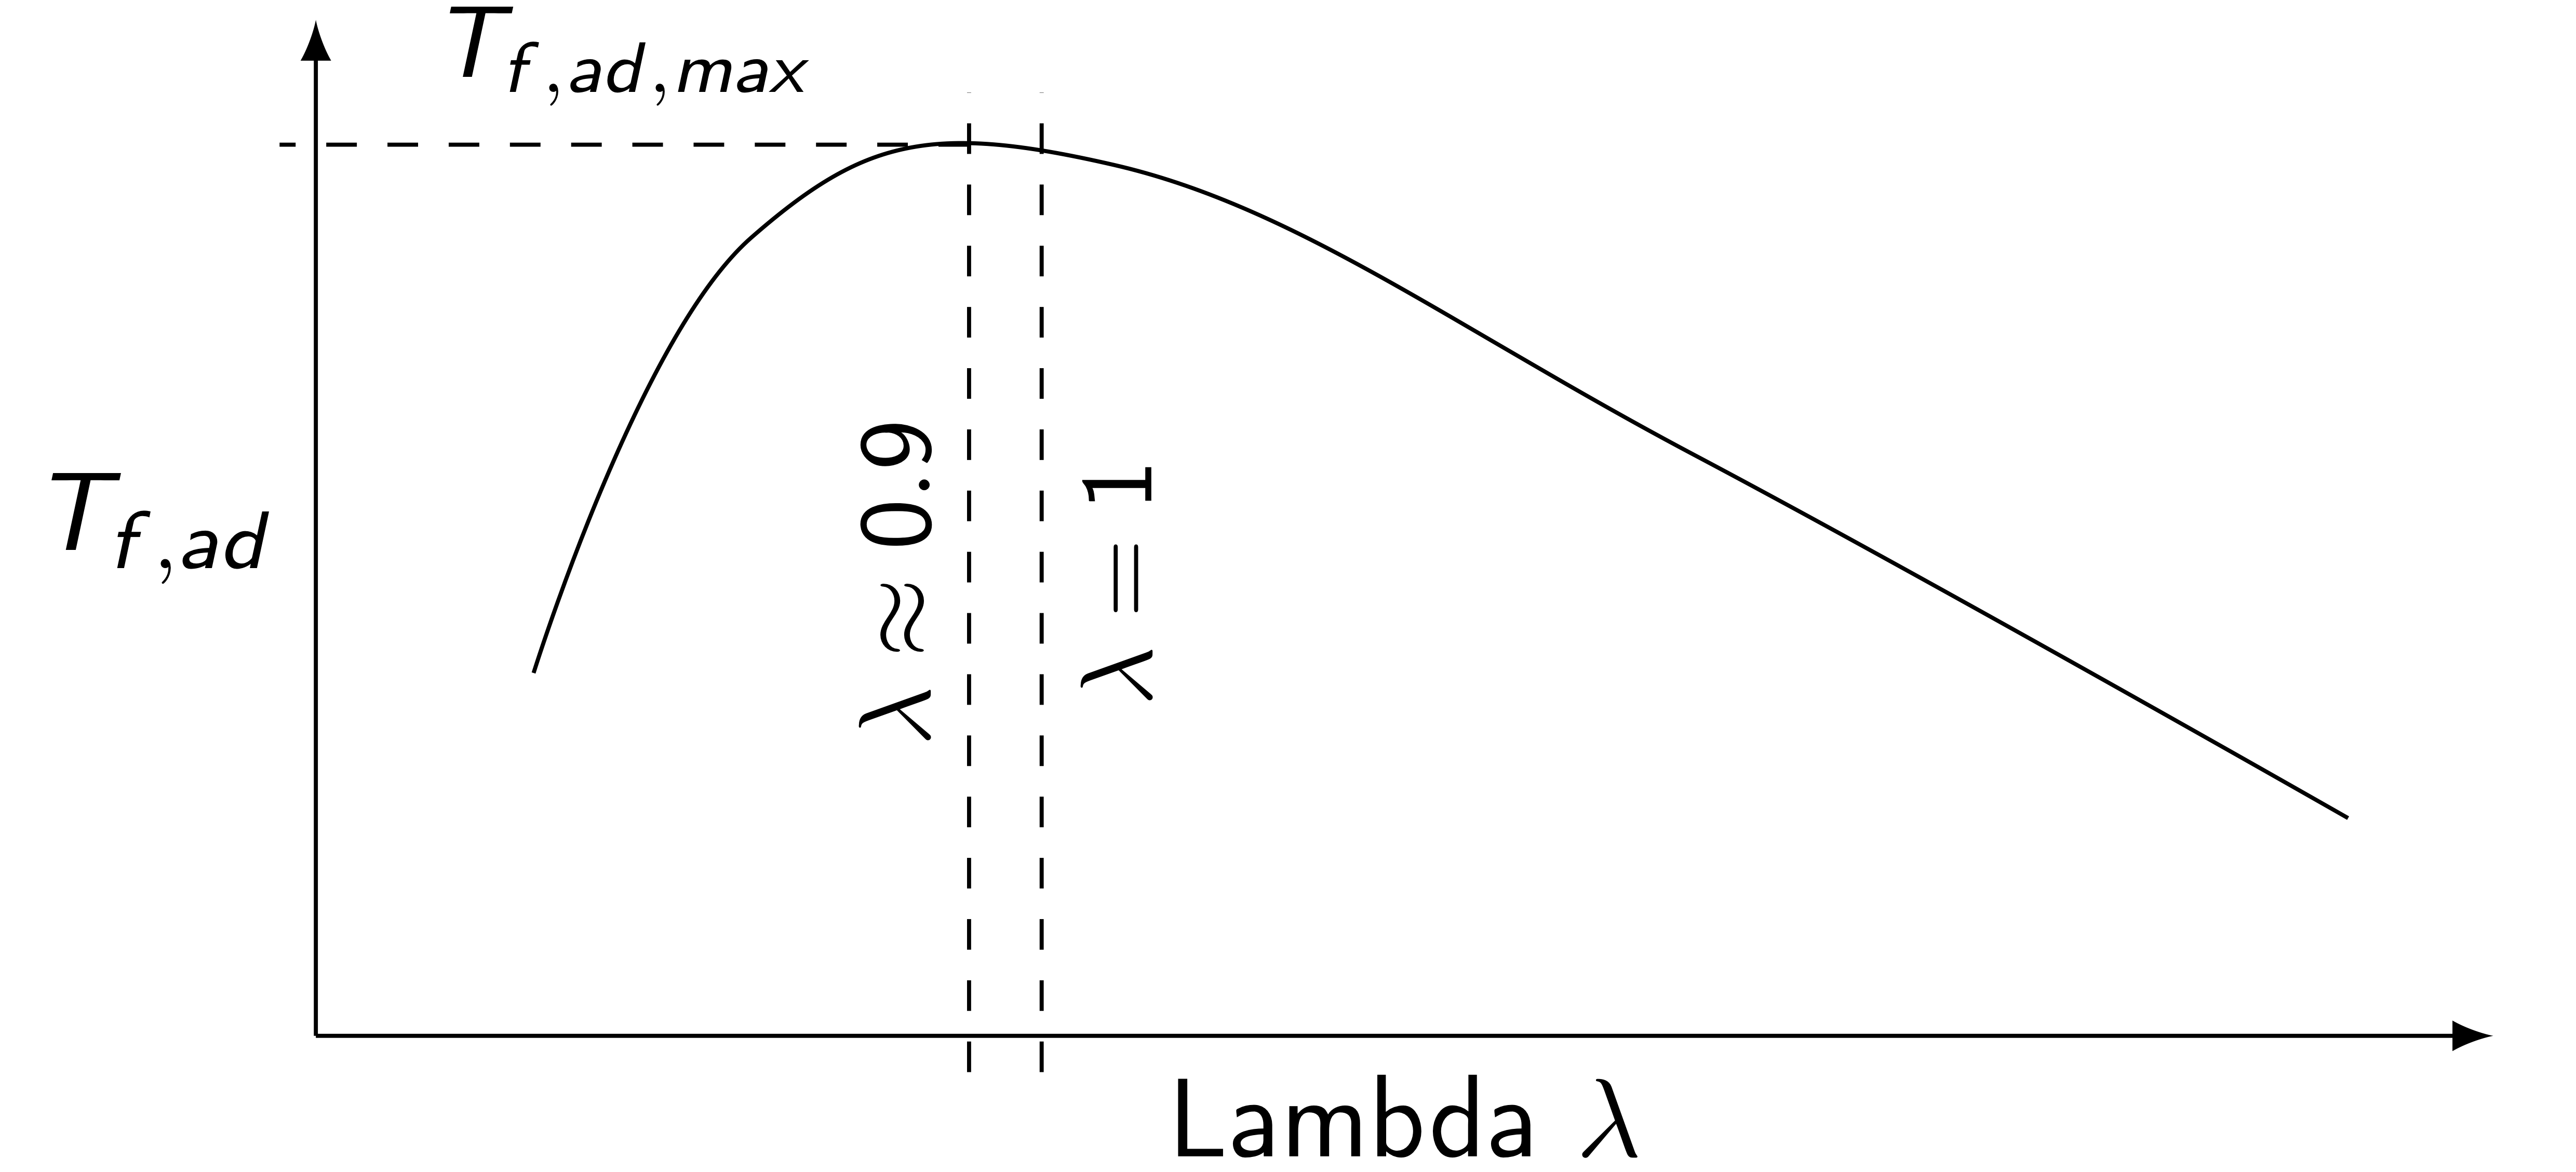
\includegraphics[width=8cm]{Bild02_Summary1_THDII}
F"ur $\lambda < 1$: Weniger W"arme und f"ur $\lambda > 1 $ gilt: zu viel ``Ballast-Luft''. Je mehr Inertgase, umso kleiner ist $T_{f,ad}$ (Aufheizung der IG). Je gr"osser der $c_p$-Wert des IG, desto mehr sinkt $T_{f,ad}$



\subsubsection*{Vorgehen f"ur Aufgaben mit adiabater Flammtemperatur}
\begin{itemize}
\item 1. HS f"ur offene Systeme: $\Delta H = Q - W$: da System adiabat, gilt $Q = 0$, es wird keine Arbeit verrichtet, also $\Delta H = 0$ $\rightarrow$ Vernachl"assigung von kin. und pot. Energie
\item $\sum_{Produkte} \tilde{h} = \sum_{Edukte} \tilde{h} $
\item $\sum_{Ed} v'_j (h_f^{0} + h(\textcolor{blue}{T_{Ed}}) - h_j(T_{ref}) ) =  \sum_{Prod} v''_j (h_f^{0} + h(\textcolor{red}{T_{f,ad}}) - h_j(T_{ref}) )$ wobei $v'_j$ und $v''_j$: st"ochiometrischen Koeffizienten
\item Umstellen ergibt (Rearranging)
\item $ \sum_{Ed} v'_j (h_f^{0} + h(\textcolor{blue}{T_{Ed}}) - h_j(T_{ref}) ) - \sum_{Prod} v''_j (h_f^{0} - h_j(T_{ref}) ) = \sum_{Prod} v''_j h(\textcolor{red}{T_{f,ad}})$
\item Linke Seite (LHS) bekannt aus Tabellen, rechte Seite (RHS) gesucht
\item Erste Sch"atzung von $T_{f,ad} \approx T_{Ed} +2000 K$
\item LHS ausrechnen
\item Gesch"atzte Temperatur in RHS einsetzen
\item Falls LHS $>$ RHS $\rightarrow T_{f,ad}$ h"oher sch"atzen
\item Sonst $\rightarrow T_{f,ad}$ tiefer sch"atzen
\item 3 Enthalpien mit LHS Zwischenwert $\rightarrow$ 2 $T_{f,ad}$ $\rightarrow$ $\textcolor{red}{T_{f,ad}}$ interpolieren
\end{itemize}



\subsection*{Heizwert}
Wasser liegt nach Verbennung entweder fl"ussig oder gasf"ormig vorliegen $\rightarrow$ Zwei verschiedene Bindungsenthalpien!
\begin{itemize}
\item Heizwerte sind die Reaktionsenthalpien unter Standardbedingungen
\item Oberer Heizwert $H_O$: Wasser fl"ussig
\item Unterer Heizwert $H_U$: Wasser gasf"ormig
\item $H_O > H_U$, da Verdampfungsenthalpie genutzt werden kann, sodass Wasser fl"ussig wird
\item Diese zus"atzliche Energie m"ussen wir bei der Gesamtenergiebetrachtung mitber"ucksichtigen 
\item Falls nicht weiter spezifiziert $\rightarrow$ immer $H_U$ verwenden
\item $H_{U,O} = -h_{R}^0 = \frac{-\bar{h}_{R}^0}{M_{fuel}}  \rightarrow [\frac{kJ}{kg}]$ 
\item Heizleistung: $P=H_{U,O}\cdot \dot{m}_{fuel} \quad [kW]$
\item Oft n"utzlich $\dot{Q} = \dot{m} c_p \Delta T$
\item $H_O = H_U + h_{fg}$ wobei $h_{fg} :=$ Verdampfungsenthalpie
\end{itemize}





\subsection*{Exhaust Gas Recirculation / Abgasr"uckf"uhrung}
Idee: Unter hohen Temperaturen kommt es zu Dissoziationsreaktionen, bei denen unerw"unschte Schadstoffe entstehen. L"osung: Senkung der adiabaten Flammtemperatur, weniger Schadstoffe.
\begin{equation}
X_{EGR}= \frac{\dot{n}_{EGR}}{\dot{n}_{net}} = \frac{{n}_{EGR}}{{n}_{net}} = \frac{n_x}{1+n_x} 
\end{equation}
$\lambda \geq 1$
\begin{itemize}
\item \ce{C_xH_y + \lambda (x +$\frac{y}{2}$) (O2 + 3.76 N2) + n_x [x CO2 + $\frac{y}{2}$ H2O + (\lambda -1) (x + $\frac{y}{4}$) O2 + 3.76 \lambda (x +$\frac{y}{4}$) N2] -> (1 + n_x) [x CO2 + $\frac{y}{2}$ H2O + (\lambda -1) (x + $\frac{y}{4}$) O2 + 3.76 \lambda (x +$\frac{y}{4}$) N2]}
\end{itemize}
$\lambda < 1$
\begin{itemize}
\item \ce{C_xH_y + \lambda (x +$\frac{y}{2}$) (O2 + 3.76 N2) + n_x [(1 - \lambda) C_xH_y + \lambda x CO2 + $\frac{\lambda y}{2}$ H2O + 3.76 \lambda (x +$\frac{y}{4}$) N2] -> (1 + n_x) [(1 - \lambda) C_xH_y + \lambda x CO2 + $\frac{\lambda y}{2}$ H2O + 3.76 \lambda (x +$\frac{y}{4}$) N2]}
\end{itemize}





\section*{Gibbs-Enthalpie / Freie Enthalpie}
ist ein Mass f"ur die nutzbare Energie einer Reaktion
\begin{itemize}
\item allgemein: $G(T,p) = H - T \cdot S \quad [kJ]$
\item ideale Gase: $g_i(T,p) = g^0_{f,i} + RT\cdot ln(\frac{p_i}{p_{ref}}) \quad [\frac{kJ}{kg}]$
\end{itemize}
"Anderung der Freien Enthalpie:
\begin{itemize}
\item Gesamtreaktion: $\Delta G = \Delta{H} - \Delta S \cdot T = \sum(v''_j - v'_j) g_j$
\item Differentiell: $dG= Vdp - SdT + \sum \mu_i dn_i$ ($Vdp \approx 0$)
\end{itemize}



\subsection*{Begrifflichkeiten: Enthalpie und Gibbs-Energie}
\begin{itemize}
\item $\Delta H < 0$ exotherm
\item $ \Delta H > 0 $ endotherm
\item $ \Delta G < 0 $ exergon
\item $\Delta G > 0 $ endergon
\end{itemize}

\subsection*{1. HS f"ur offene Systeme}
Aus Thermo I gilt f"ur station"are Systeme:
\begin{equation}
\dot{Q} -\dot{W}_S = \sum_P \dot{m}_e h_e - \sum_E \dot{m}_i h_i = \Delta \dot{H} |_{E\rightarrow P}
\end{equation}
Wir schreiben unsere chemischen Verbrennungsprozesse immer so, dass unser Brennstoff den st"ochiometrischen Koeffizienten 1 besitzt. Der Rest ist im Verh"altnis dazu bemessen, d.h. pro mol Brennstoff haben an der Gesamtreaktion so und so viele andere Reaktanden einen Anteil, d.h. in einem Kontrollvolumen gilt:
\begin{equation}
\frac{\dot{Q}}{\dot{n}_{fuel}} - \frac{\dot{W}_S}{\dot{n}_{fuel}} = \sum_P n_e \bar{h}_e - \sum_E n_i \bar{h}_i
\end{equation}
Hierbei gilt noch $\dot{n}_{fuel} = \frac{\dot{m}_{fuel}}{M_{fuel}}$

\subsection*{1.HS f"ur geschlossene Systeme}
Hier gilt ebenfalls aus Thermo I:
\begin{equation}
\Delta E = Q-W = \Delta U
\end{equation}
wenn KE und PE vernachl"assigbar. Bei idealen Gasen gilt ebenfalls:
\begin{equation}
\bar{u} = \bar{h} - \bar{R} T = \bar{h}_f^0 + \bar{h}(T) - \bar{h}(T_{ref})-\bar{R}T
\end{equation}
daraus folgt
\begin{equation}
\begin{split}
Q-W = \sum_P n \left( \overline{h}_{f}^{0} + \overline{h}(T) - \overline{h}(T_{ref})\right) \\ - \sum_E n \left( \overline{h}_{f}^{0} + \overline{h}(T) - \overline{h}(T_{ref})\right) - \bar{R} T_P \sum_P n + \bar{R} T_E \sum_R n
\end{split}
\end{equation}



\section*{Chemisches Gleichgewicht}
{\bf{Eine chemische Reaktion minimiert die die Gibbs-Energie}}
\newline
Ein System befindet sich im Gleichgewicht, sobald
\begin{equation}
dG(T,p) = Vdp - S(T,p) dT + \sum \mu_i dn_i=0
\end{equation}
\begin{itemize}
\item Das GGW ist abh"angig von Temperatur und Druck
\item Es stellen sich GGW-Stoffmengen ein
\begin{equation}
\sum_{Ed} n'_i \bar{g}_i = \sum_{Prod} n''_i \bar{g}_i 
\end{equation}
\end{itemize}
{\bf{Nun k"onnen die Gleichgewichtskonzentrationen bestimmt werden}}


\subsection*{Gleichgewichtskonstante $K_p$}
Gegebene Reaktion
\begin{equation}
\sum_{Ed} \nu'_i M_i \rightleftharpoons \sum_{Prod} \nu''_i M_i
\end{equation}
{\bf{Formel f"ur Partialdr"ucke $p_i$!}}
\begin{equation}
K_p(T) = exp \left(-\frac{\Delta G_0}{RT} \right) = exp \left(-\frac{\Delta \overline{G}_0}{\overline{R} T} \right)
\end{equation}
Wobei $\overline{\Delta G}_0 = \sum \nu''_i \overline{g_i}^0 - \sum \nu'_i \overline{g_i}^0 = \sum (\nu''_i-\nu'_i) \bar{h}_i - T \sum (\nu''_i -\nu'_i) \bar{s}^0$ bei Druck $p_{tot}=p_{ref}$
\begin{equation}
K_p(T) = \prod_i \frac{(p_i/p_{ref})^{v''_i}}{(p_i/p_{ref})^{v'_i}} = \left( \prod_i \frac{n_i^{v''_i}}{n_i^{v'_i}}\right) \left( \frac{p_{tot}}{n_{tot} \cdot p_{ref}} \right)^{\sum v''_i - v'_i}
\end{equation}
Umrechnung f"ur {\bf{Konzentrationen}}



\begin{equation}
\begin{split}
K_c(T) &= K_p(T) \cdot \left( \frac{p_{ref}}{\overline{R}T} \right) ^{\sum v''_i-v'_i} \\\ 
&= \prod_i \frac{c_i^{\nu''_i}}{c_i^{\nu'_i}}
\end{split}
\end{equation}
Umrechnung f"ur {\bf{Stoffmengen}}



\begin{equation}
K_n(T) = K_p(T) \cdot \left( \frac{n_{tot}\cdot p_{ref}}{p_{tot}} \right) ^{\sum v''_i-v'_i}
\end{equation}

\subsubsection*{Beispiel - Dissoziation}
Wieviel Stickstoff dissoziiert bei 3000K und 2 bar? \ce{N_2 <=> 2N}
\begin{itemize}
\item Diss.gleichung in Reaktionsgleichung umschreiben: \ce{N_2 -> a $\cdot$ 2N + b$\cdot$ N_2}
\item Massenerhaltung: $a+b=1 \rightarrow a=$ dissipierter Anteil \ce{N2}, $b=$ Rest 
\item Stoffmengen $(2a),b$ und st. Koeff. aus Dissoziationsgl
\item In Reaktionsgleichung: \ce{N_2 -> 2a N + (1-a) N2}
\item Ergebnis in $K_p$ (Partialdruck gegeben/gefragt) einsetzen, sonst anderer $K_x$
\item $K_p = \frac{(2a)^2}{(1-a)^1} \cdot \frac{2bar}{[2a + (1-a)]\cdot 1bar}$
\item Aus Tab A-32 $\rightarrow K_p$ auslesen und ggf. in andere $K_x$ umrechnen. Achtung: 10er-Logarithmus! $\rightarrow 10^{Tabellenwert}$
\item Mit dem Taschenrechner nach $a$ bzw. $b$ aufl"osen, wichtig ist: $a$ muss als Ergebnis sehr klein werden! TR-Funktion: $nsolve(....,a)$ oder $solve(....,a)$
\item Es folgt $n_{tot}=2a+(1-a)$ und daraus die Partialdr"ucke
\end{itemize}

\subsubsection*{Gleichgewichtsanteile bei Verbrennungen}
\begin{itemize}
\item \ce{ CO + 0.5 O2 + 1.88 N2 -> CO2 +1.88 N2}
\item Dissoziationsgleichung: \ce{CO_2 <=> CO + 0.5 O_2}
\item \ce{CO + 0.5 O2 + 1.88 N2 -> a CO + a 0.5 O2 + (1-a) CO2 + 1.88 N2} sind die Mengenanteile vor der Einstellung des GGW
\item $n_{net} = a + 0.5 a + (1-a) + 1.88$
\item Stoffmengen: $n_{\ce{CO}}=a$, $n_{\ce{O2}}=\frac{a}{2}$, $n_{\ce{CO2}}=1-a$
\item St"ochiometrische Koeff: Aus Dissoziationsgleichung bzw. GGW
\item $\Delta H_R$ ist aus der GGW-Gleichung
\end{itemize}

\subsection*{Weiteres zu Chemischen Gleichgewichten}
{\bf{Gleichgewichtskonstanten sind temperaturabh"angig!}}
\begin{itemize}
\item $K \gg 1$: Mehr Produkte
\item $K \approx 1$: Keine dominante Richtung
\item $K \ll 1$: Mehr Edukte
\item Es gibt Aufgaben, bei denen Konzentration gegeben ist und Temperatur gesucht ($K_p$)
\item Es gibt Aufgaben, bei denen die Temperatur gegeben ist und Konzentrationen gesucht werden! (Beispiele zuvor)
\end{itemize}

\subsection*{Prinzip von Le-Chatelier}
{\bf{Ein Gleichgewicht weicht "ausseren Zw"angen aus}}
\newline
\newline
\ce{2 A + 3 B <=> C + 2 D} $ \quad \Delta H<0$
Wie verschiebt sich das GGW, wenn: 
\begin{itemize}
\item ...der Druck erh"oht wird? $\rightarrow$ betrachte st"och. Koeffizienten: $2 + 3 > 1 + 2 \rightarrow$ GGW verschiebt sich nach rechts (mehr Produkt)
\item ...die Temperatur steigt? $\rightarrow$ betrachte Reaktionsenthalpie: $\Delta H < 0$: exotherm, d.h. GGW verschiebt sich nach links (Temp.erh"ohung beg"unstigt endotherme Reaktion, siehe n"achste Seite)
\item ...weiteres A oder B hinzugef"ugt wird? $\rightarrow$ GGW geht nach rechts, Edukt"uberschuss beg"unstigt mehr Produkte
\end{itemize}
{\bf{Jedoch bleibt wie immer die Gleichgewichtskonstante nur temperaturabh"angig! Sie "andert sich bei einer Konzentrations- oder Druck"anderung nicht}}

\subsection*{Adiabatische Flammtemperatur im Gleichgewicht}
Hier werden zwei uns bekannte Verfahren kombiniert. Dies bringt jedoch ein Problem mit sich, wenn wir zuerst auf dem uns bekannten Weg die Flammtemperatur bestimmen und danach die via $K_p$ nach $a$ aufl"osen, ergibt dies eine neue Reaktionsgleichung und daraus resultierend eine neue Flammtemperatur. Dies ist nun ein {\bf{Fixpunkt-Problem}}. Wir k"onnen das ganze Prozedere immer wieder durchf"uhren, wobei wir uns immer n"aher der korrekten L"osung ``anschleichen''.


\section*{Exergie}
ist die maximal nutzbare Energie bis zum vollst"andigen Ausgleich mit der Umgebung. Beachte: Da immer gerechnet mit wird molaren Gr"ossen $\rightarrow$ pro mol Brennstoff!
\newline
\newline
Exergiebilanz f"ur geschlossene Systeme
\begin{equation}
Ex = W_{nutz, rev} = U - U_0 + p_0 \cdot \left( V - V_0 \right) - T_0\cdot \left( S - S_0 \right)
\end{equation}
Str"omung
\begin{equation}
\dot{Ex} = \dot{W}_{nutz, rev} = \dot{m} \cdot \left( h-h_0 -T_0 (s-s_0) \right)
\end{equation}
\begin{equation}
\Delta{E_x} |_{1\rightarrow 2} = \dot{m} (h_2-h_1 - T_0(s_2-s_1))
\end{equation}

Exergiebilanz f"ur offene Systeme
\begin{equation}
\begin{split}
\frac{d}{dt} Ex = \sum_{in} \dot{m}_{in} ex_{in} - \sum_{out} \dot{m}_{out} ex_{out} + \\ + \left( 1- \frac{T_0}{T_G} \right) \dot{Q} -\dot{W} - \dot{Ex}_{Verlust}
\end{split}
\end{equation}

Exergieverlust ($\dot{S}_{erz} = \dot{S}_{irr}$, oft $\frac{d}{dt} S = 0$) berechne zuerst $\dot{S}_{irr}$!
\begin{equation}
\begin{split}
\dot{Ex}_{Verlust} = T_0 \cdot \dot{S}_{erz} \\ \dot{S}_{irr}= \frac{d}{dt} S - \sum_i \frac{\dot{Q}_i}{T_{G,i}} + \sum_{out} \dot{m}_{out} s_{out} -\sum_{in} \dot{m}_{in} s_{in}
\end{split}
\end{equation}

Entropiedifferenzen (ideale Gase)
\begin{equation}
s_i(T,p_i) = s^0_i(T) - R \cdot ln\left(\chi_i \frac{p_{tot}}{p_{ref}}\right) \quad \left[ \frac{kJ}{K\cdot kg}\right]
\end{equation}
\begin{equation}
\begin{split}
s_2 - s_1 &= s^0(T_2) - s^0(T_1) - R \cdot ln \left( \frac{p_2}{p_1} \right) \\\ 
&\approx c_p \cdot ln \left( \frac{T_2}{T_1} \right) - R \cdot ln \left( \frac{p_2}{p_1} \right) \\\
& \approx c_v \cdot ln \left( \frac{T_2}{T_1} \right) + R \cdot  ln \left( \frac{v_2}{v_1} \right)
\end{split}
\end{equation}

Entropiedifferenzen (Feststoffe und inkomp. Fl"ussigkeiten, $c_{avg}$ Durchschnitt der c-Werte bei $T_2$, $T_1$)
\begin{equation}
s_2 - s_1 \approx c_{avg} \cdot ln \left( \frac{T_2}{T_1} \right)
\end{equation}

\section*{Van't Hoff Gleichung}
Idee: Quantitative Temperaturabh"angigkeit von $K_p$
\begin{equation}
\frac{d}{dT} \left( ln (K_p) \right) = \frac{\Delta H_R(T)}{RT^2}
\end{equation}
Dies folgt aus der Gleichgewichtsbedingung $dG=0$. Unter der Annahme, dass $\Delta H_R \neq f(T)$ folgt
\begin{equation}
ln \left( \frac{K(T_2)}{K(T_1)} \right) = - \frac{\Delta H_R}{R} \left( \frac{1}{T_2} - \frac{1}{T_1} \right)
\end{equation}
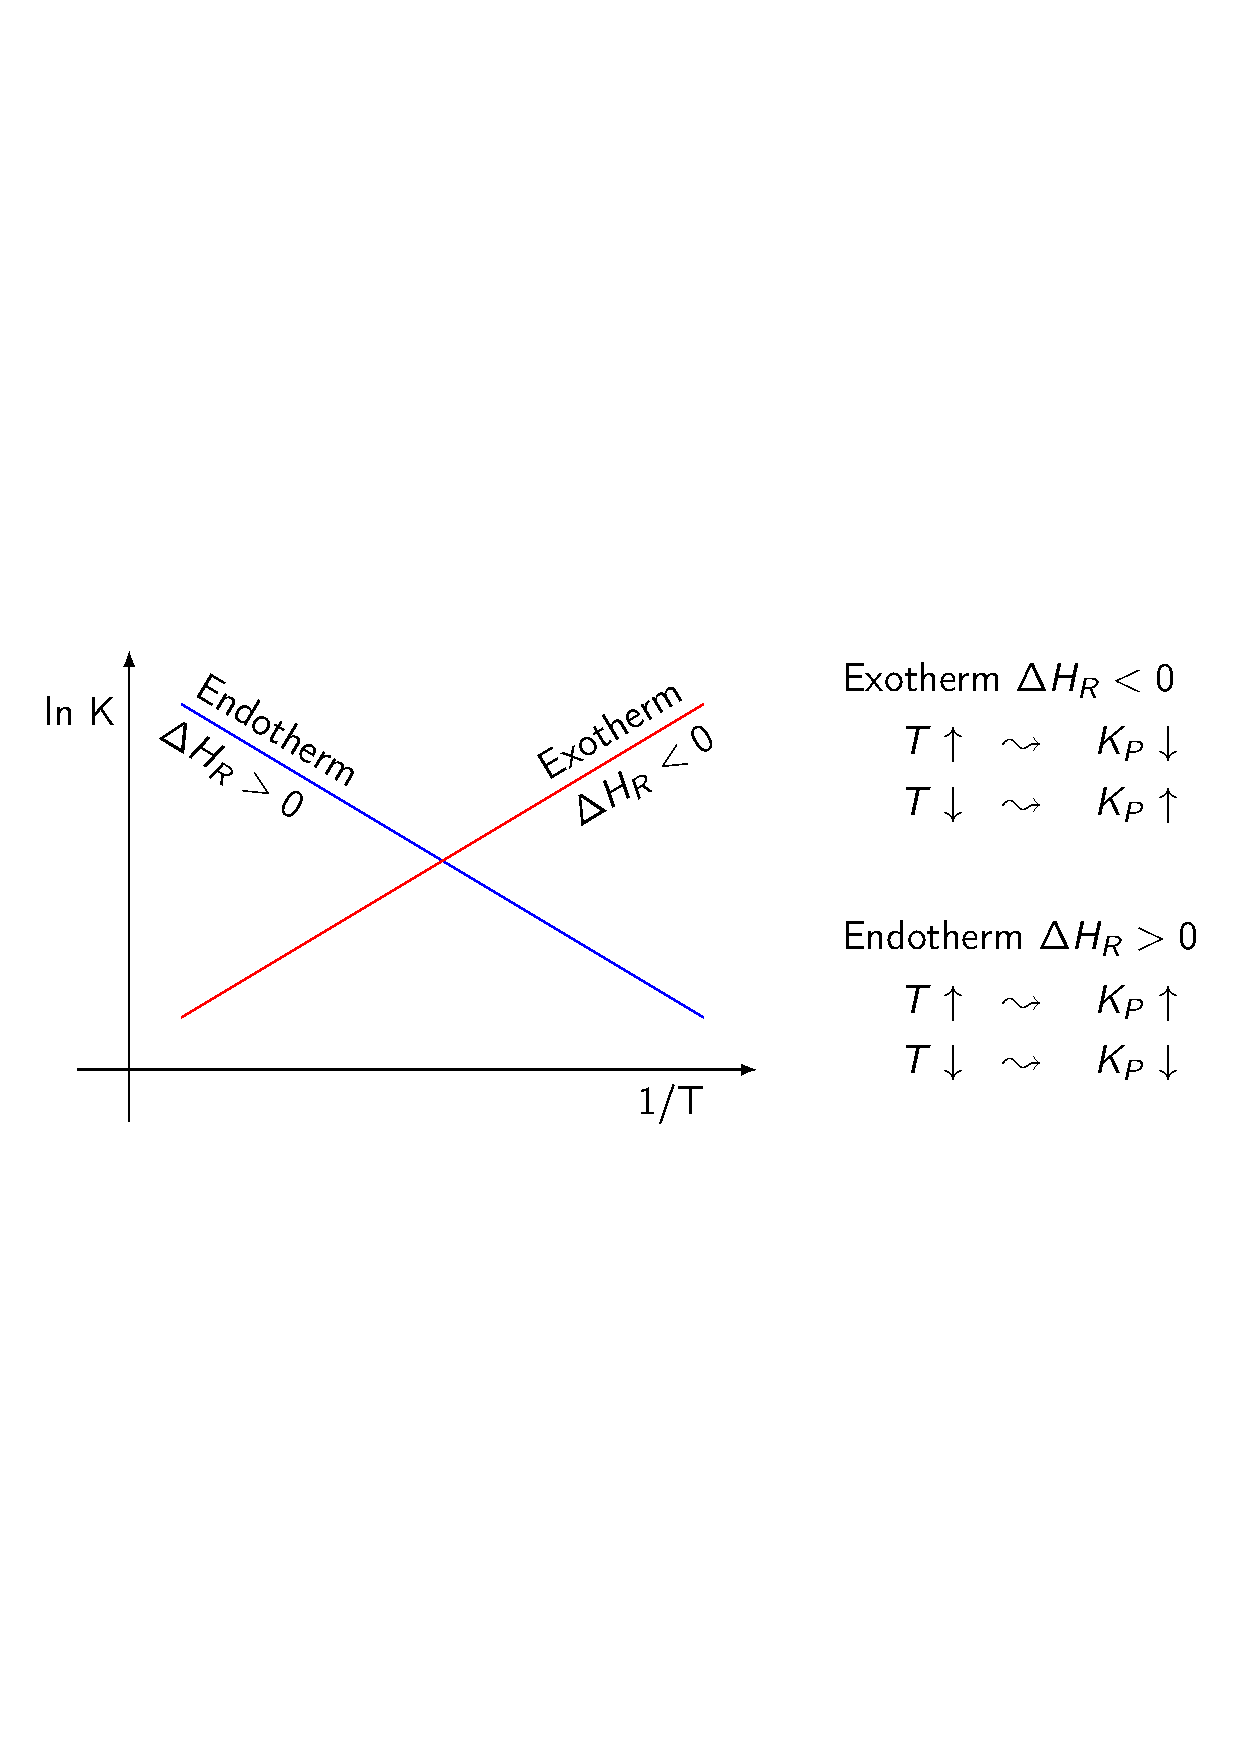
\includegraphics[width=8cm]{Bild03_Summary1_THDII}


\section*{Brennstoffzellen}
werden verwendet, um thermische Energie in elektrische Energie umzuwandeln
\subsubsection*{Redoxreaktionen: "Ubertragung von Elektronen}
\begin{itemize}
\item Elektronenabgabe: Oxidation, Minuspol, Anode (OMA)
\item Elektronenaufnahme: Reduktion, Pluspol, Kathode
\end{itemize}

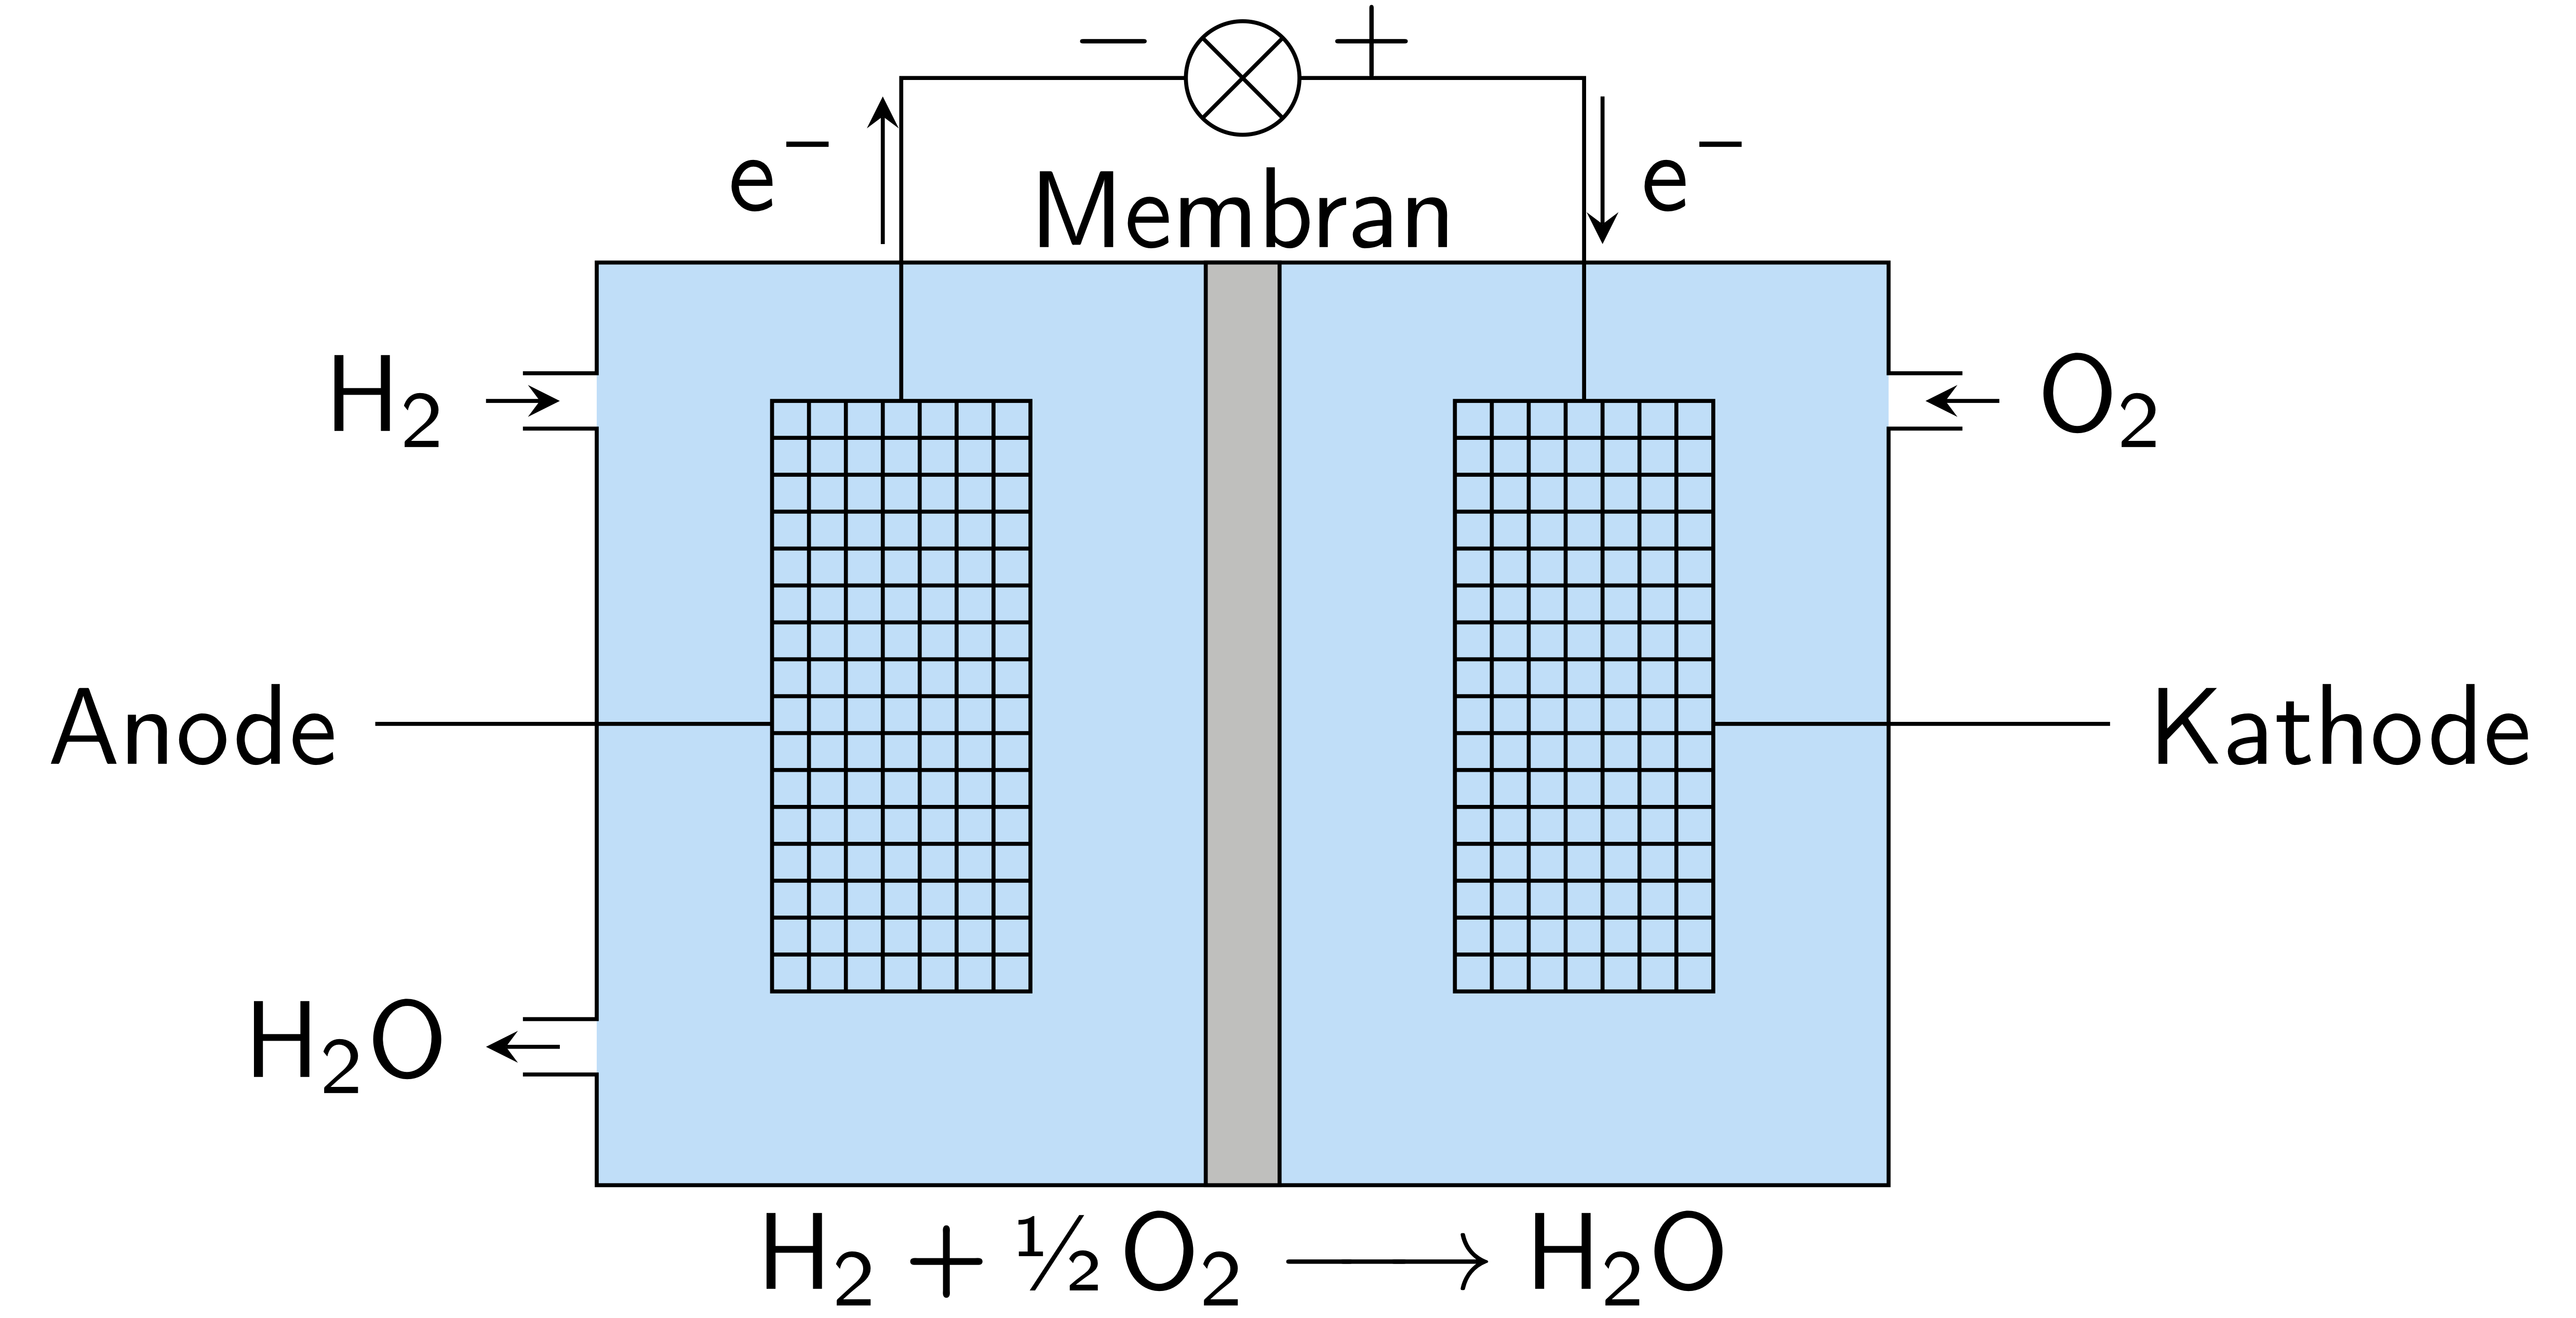
\includegraphics[width=8cm]{Bild04_Summary1_THDII}

\subsubsection*{Beispiel: Reaktion von Wasser- und Sauerstoff zu Wasser} 
\begin{center}
\ce{H2^0 + 1/2 O2^0 -> H2^{1+}O^{2-}}
\end{center}

Aufteilen der Globalreaktion in Anode und Kathode

\begin{tabular}{l*{5}{l} r}
Global: & $\quad$ & \ce{H2} & +\ce{1/2 O2} & $\longrightarrow$ & \ce{H2O} & $\quad$ \\
\hline
Anode: & $\quad$ & \ce{H2} & + \ce{ 2 OH^-} & $\longrightarrow$ & \ce{2H2O} & + \textcolor{blue}{2 $e^-$} \\
Kathode: & \ce{1/2 O2} + & \ce{2H2O} & +\textcolor{blue}{2 $e^-$} & $\longrightarrow$ & \ce{2OH^-} & +\ce{H2O} \\
\end{tabular}

\begin{equation}
\boxed{I = F\cdot N_e \cdot \dot{n}_{Brenn} \cdot \eta_I = \left(\dot{n}_e \cdot F \right) \eta_I}
\end{equation}

Es werden $N_e=\textcolor{blue}{2e^-}$ frei $\longrightarrow$ $F$=Faraday-Konstante, $I$=Strom
\newline
\newline
Wichtig: Immer zuerst bestimmen, welcher Teil Anode und welcher Kathode ist. Die Anzahl der "ubertragenen Elektronen kann aus der Globalreaktion abgeleitet werden. Diese ist essentiell f"ur die sp"atere Rechnung. Mit \ce{OH^-} und \ce{H2O} werden die einzelnen Teilreaktionen ausgeglichen.

\subsubsection*{Beispiel: S"auren in Redoxgleichungen}
\begin{center}
\ce{H^{1+}C^{2+}O^{2-}O^{2-}H^{1+} + 1/2 O2^0 -> C^{4+}O2^{2-} + H2^{1+}O^{2-}}
\end{center}
Der Ausgleich durch Elektronen resultiert aus der Umlagerung der Bindungselektronen in der S"aure
\begin{tabular}{l*{5}{l} r}
Global: & $\quad$ & \ce{HCOOH}& +\ce{1/2 O2} & $\longrightarrow$ & \ce{CO2} & \ce{H2O} \\
\hline
Anode: & $\quad$ & \ce{HCOOH} & $\longrightarrow$  & \ce{2H+}  & +\ce{CO2} & + \textcolor{blue}{2 $e^-$} \\
Kathode: & \ce{1/2 O2} + & \ce{2H+} & +\textcolor{blue}{2 $e^-$} & $\longrightarrow$ & $\quad$ & +\ce{H2O} \\
\end{tabular}


\subsection*{N"utzliche Formeln f"ur Brennstoffzellen}
\begin{itemize}
\item 1. HS: $\dot{Q} + P_Z = \dot{n}_{fuel}\cdot\Delta H_R$ bzw. $\dot{n}_{fuel} \cdot -H_U$
\item Kalorische Zellspannung: $U_H(T) = -\frac{\Delta H_R}{N_e \cdot F}$
\item Rev. Spannung (Klemm-): $U_{rev} = -\frac{\Delta G_R}{N_e \cdot F}$
\item Normierter Stromfluss: $\tilde{I} = \frac{I}{I_{max}}$
\item Leistung der Zelle: $P_Z = -U(\tilde{I})\cdot I = -U(\tilde{I})\cdot \tilde{I} \cdot I_{max}$
\item Maximale Leistung: Randbedingungen ($I=0$, $I=I_{max} \rightarrow \tilde{I}=0$ oder $1$) oder bei $\frac{dP_Z}{dI}=0$ und $\frac{d^2P}{dI^2} < 0$
\item Umsetzungsgrad: $\eta_I = \frac{\dot{n}_{fuel}}{\dot{n}_{fuel}^{*}} = \frac{I}{N_e\cdot F \cdot \dot{n}_{fuel}^{*}}$
\item $\dot{n}_{fuel}$ = Umgesetzter Brennstoffmolstrom
\item $\dot{n}_{fuel}^{*}$ = Zugef"uhrter Brennstoffmolstrom
\item Energetischer W.grad: $\eta_Z = \eta_I \cdot U(\tilde{I})\cdot \frac{N_e \cdot F}{H_U} = \eta_I \cdot \eta_{U,H} = \eta_I \frac{P_Z}{P_Z+\dot{Q}} = \eta_I \frac{U(\tilde{I})}{U_H(T)}$
\item Stapelspannung: $U_S=N\cdot U_Z$, $P_S= N\cdot P_Z$
\item $x_Z$: Pro Zelle
\item $x_S$: Pro Stapel
\item W"armestr"ome $\dot{Q}=\dot{Q}_{rev}+\dot{Q}_{irr} = -\left[ U_H - U(\tilde{I}) \right] \cdot I$
\item $\dot{Q}_{rev}= -\left[ U_H - U_{rev} \right] \cdot I$
\item $\dot{Q}_{irr} = - \left[ U_{rev} - U(\tilde{I}) \right] \cdot I$


\end{itemize}

\subsubsection*{N"utzliches zu Brennstoffzellen}
\begin{itemize}
\item Immer zuerst Reaktionsgleichungen aufschreiben \\ $\longrightarrow$ Teilpunkte
\item Kalorische oder auch Klemmspannung angegeben/gemessen
\item $\Delta H_R$ bzw. $\Delta G_R$ daraus ableiten
\item Danach alles andere bestimmen
\end{itemize}




\subsubsection*{Beispiele von Brennstoffzellen}
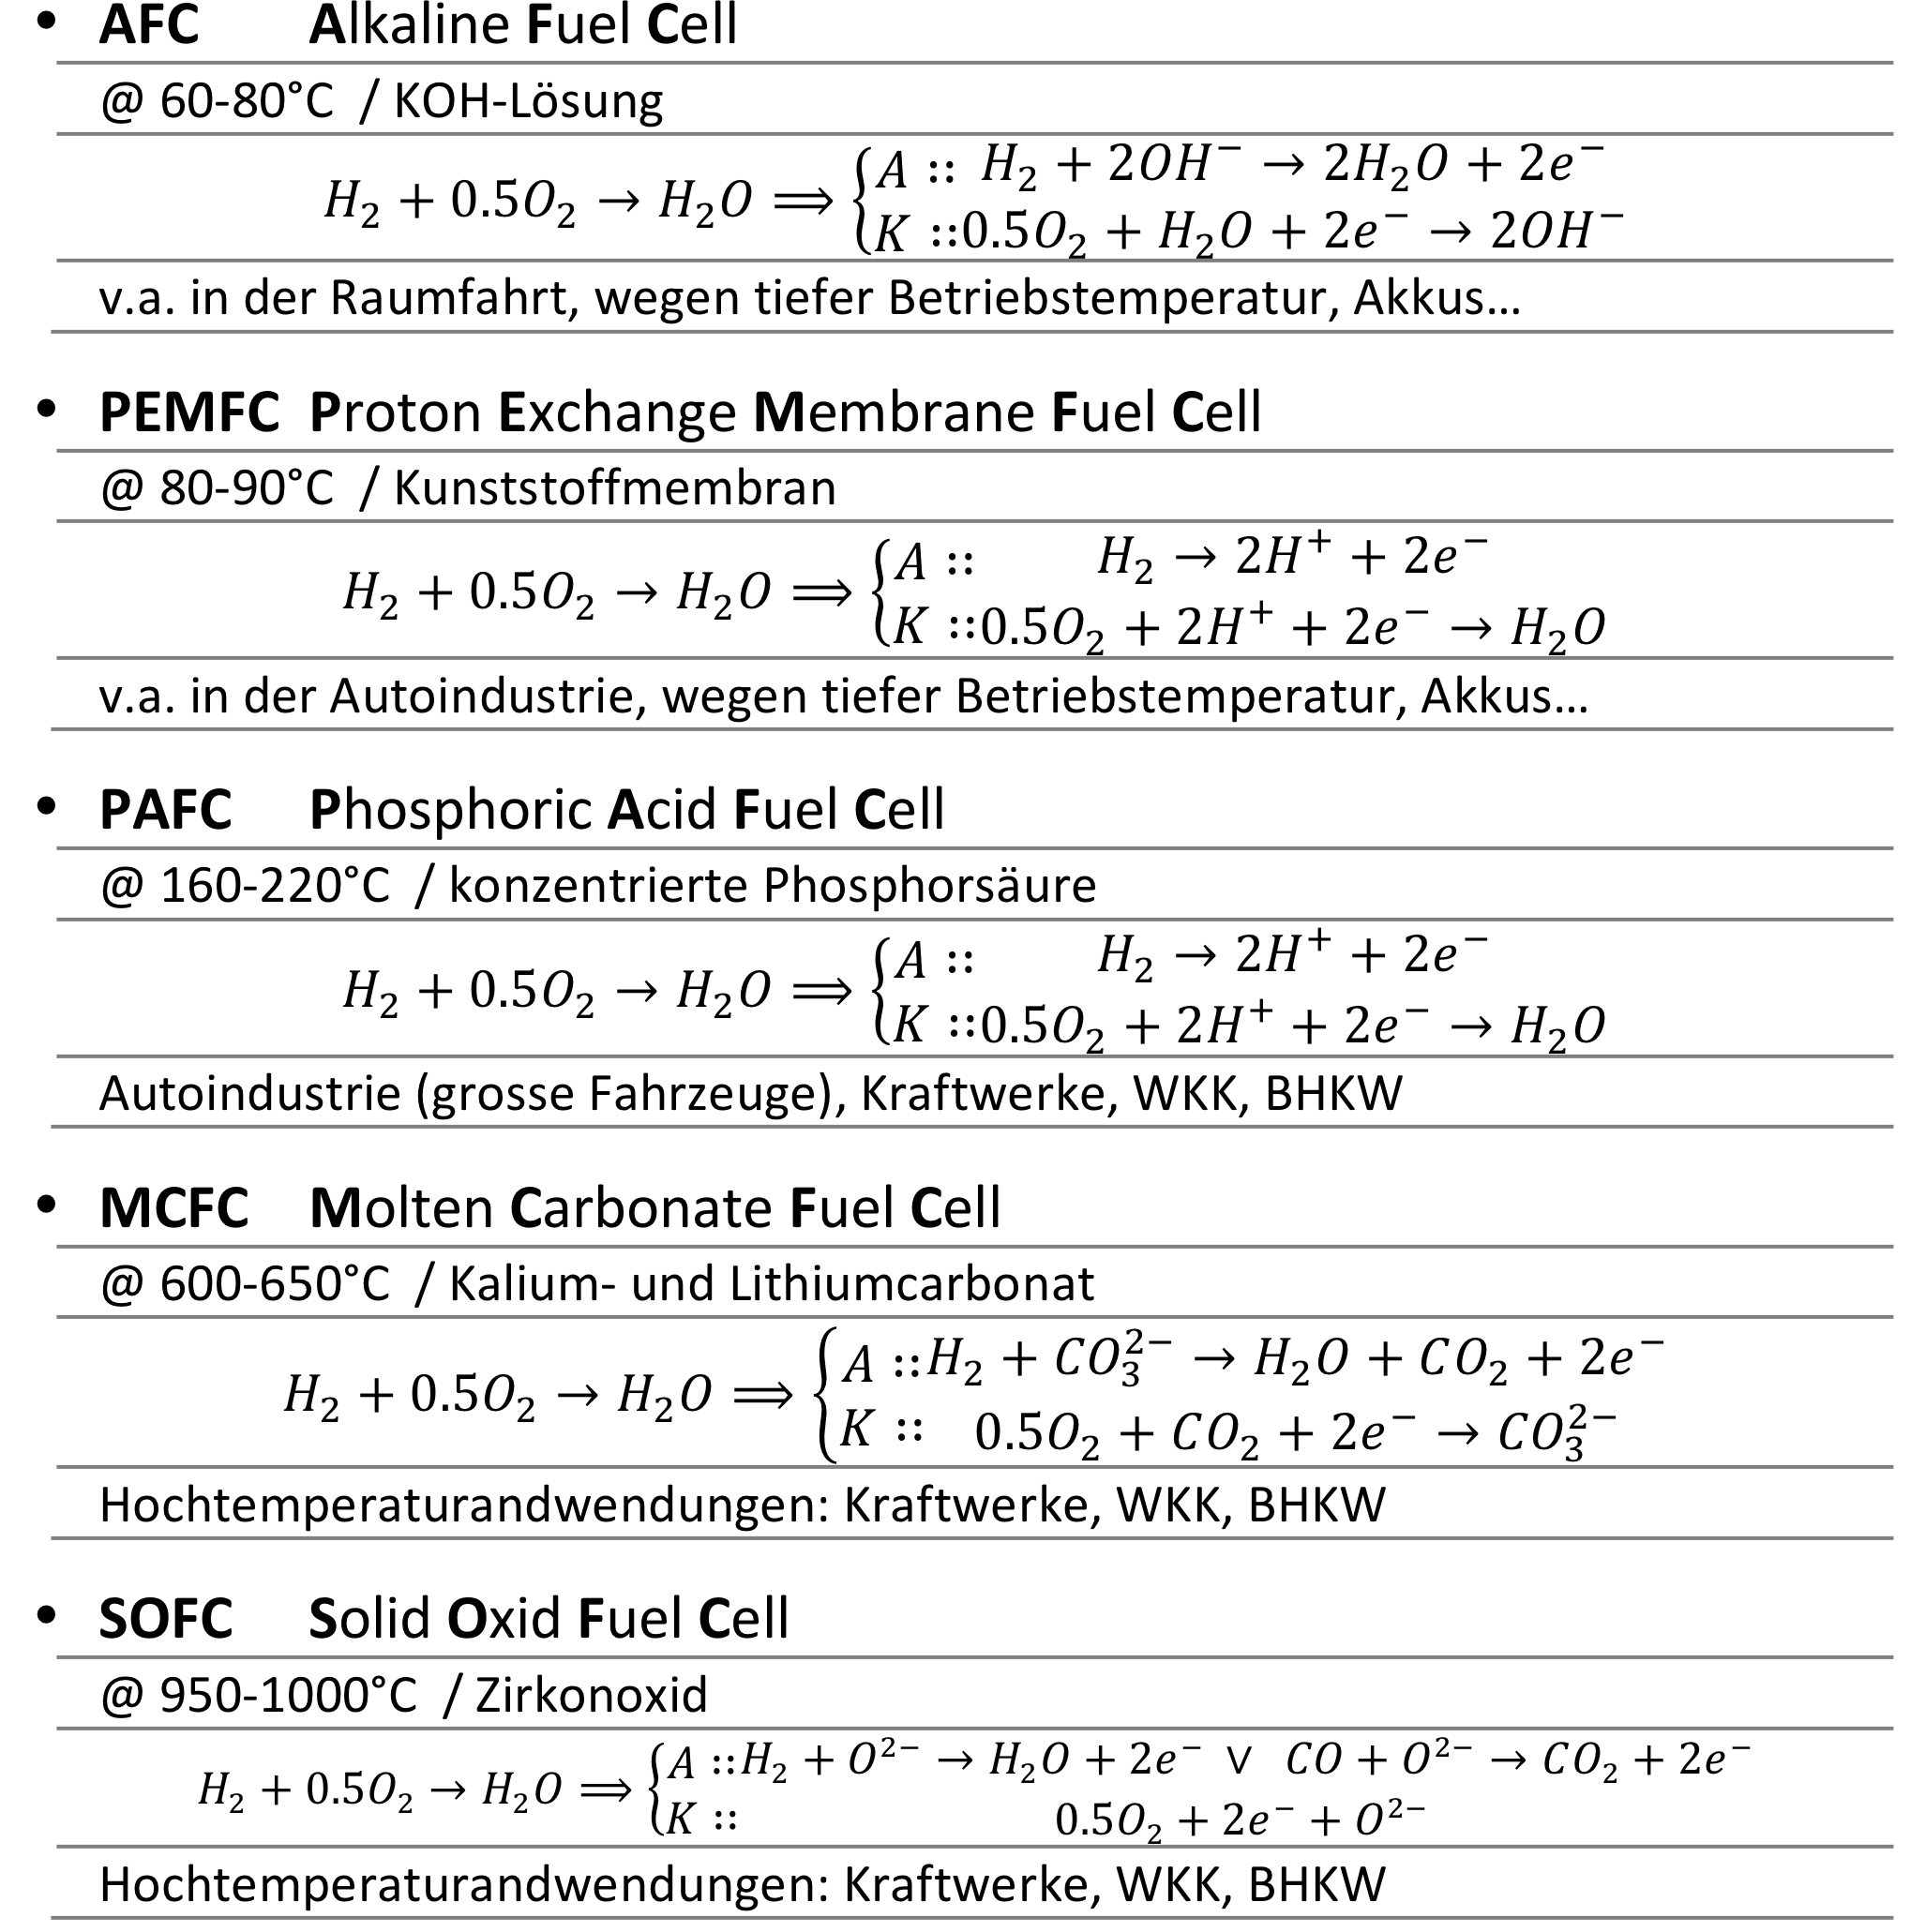
\includegraphics[width=8cm]{Bild05_Summary1_THDII}


\section*{Entropie: Wiederholung und Beispiele}

\subsection*{Vorgehen: Bestimmung der Entropie eines idealen Gasgemisches}
\begin{itemize}
\item Luft besteht zu 21\% aus \ce{O2} und 79\% aus \ce{N2}
\item $s_{Luft} = 0.21 s_{\ce{O2}} + 0.79 s_{\ce{N2}}$
\item Partialdr"ucke: $p_{Luft} = p_{\ce{O2}} + p_{\ce{N2}}$
\item Aus Entopiegleichung bei Kap. Exergie folgen die einzelnen Entropien
\item Kombinieren
\end{itemize}

\subsection*{Allgemeine Formel: Entropie eines idealen Gasgemisches}
F"ur 1 kmol der Mischung gilt:
\begin{equation}
s(p,T) = \sum_{i=1}^{N} \chi_i s^0_i(T) - R \cdot ln\left(\frac{p_{tot}}{p_{ref}}\right) - R\sum_{i=1}^{N} \chi_i ln \left( \chi_i \right)
\end{equation}
F"ur n kmol der Mischung gilt ($n_i = \chi_i \cdot n$):
\begin{equation}
n\cdot s(p,T) = \sum_{i=1}^{N} n_i s^0_i(T) - R\cdot n \cdot ln\left(\frac{p_{tot}}{p_{ref}}\right) - R\sum_{i=1}^{N} n_i ln \left( \chi_i \right)
\end{equation}

Beachte: Fl"ussigkeiten z"ahlen bei der Bestimmung der Partialbr"uche nicht! Diese haben keinen Beitrag zum Druck

\subsection*{Entropie eines ``steady-state burner", adiabat}
Aus dem Prinzip von Clausius folgt
\begin{equation}
S_2 - S_1 = \int \frac{\delta Q}{T} + S_{ir}
\end{equation}
Aus Tabllen und der Reaktionsgleichung (s.o.) folgen auf der linken Seite die Entropiedifferenz und auf der rechten Seite f"ur adiabate Brenner gerade $S_{ir}$. 

\subsection*{Nicht-adiabter Fall}
Hierbei kann man das Integral nicht mehr vernachl"assigen, es addiert sich ein Term hinzu:
\begin{equation}
S_2 - S_1 = \frac{Q}{T_G} + S_{ir}
\end{equation}
Es wird ein Teil der W"arme an die Umgebung abgegeben. Diese W"arme entspricht dem Enthalpieunterschied zwischen End- und Anfangszustand (Reaktionsw"arme) bei einer Temperatur, wo der W"arme"ubergang stattfindet.

\subsection*{3. Hauptsatz der Thermodynamik}
Die Entropie einer Substanz ist beim absoluten Temperaturnullpunkt nur dann null, wenn diese eine perfekte kristalline Struktur hat. Sonst hat sie die absolute Entropie beim Nullpunkt von $s^0(T=0)$.
Diese findet man bei Tab. A-30.

\subsection*{Allgemeine Formeln zur Bestimmung der Entropien} 
Immer Reaktionsgleichung bez"uglich ein Mol Brennstoff


\subsubsection*{Entropiebilanz: System offen, station"ar}
\begin{equation}
\begin{split}
\frac{\dot{S}_{erz}}{\dot{n}_{fuel}} = -\sum \frac{\dot{Q} / T_G}{\dot{n}_{fuel}} + \sum_{Produkte} n \left( \overline{s}^0(T) + \overline{R} ln \left(\chi_i \frac{p_{tot}}{p_{ref}} \right) \right)
\\ - \sum_{Edukte} n \left( \overline{s}^0(T) - \overline{R} ln \left(\chi_i \frac{p_{tot}}{p_{ref}} \right) \right)
\end{split}
\end{equation}
Falls $p_{reaktion} \equiv p_{tot}=p_{ref}$ und $\dot{Q} = 0$:
\begin{equation}
\frac{\dot{S}_{erz}}{\dot{n}_{fuel}} = \sum_{P} n \overline{s}^0(T) -\sum_{E} n \overline{s}^0(T) - \overline{R} ln \left( \frac{\Pi_{P} (\chi_i)^n)}{\Pi_{E} (\chi_i)^n} \right)
\end{equation}
Die $\overline{s}^0$-Werte befinden sich f"ur Brennstoffe bei 298 K in A-30, f"ur verschiedene Gase bei verschiedenen Temperaturen zwischen A-22 bis A-28. {\bf{F"ur geschlossene Systeme gelten die gleichen Bedingungen, jedoch mithilfe der offenenen Systemen l"asst sich der Exergieverlust bestimmen}}.

\subsection*{Allgemeine Formeln zur Bestimmung der chemischen Exergie}
Die chemische Exergie wird immer zur thermomechanischen Exergie hinzugef"ugt (siehe oben)

\subsubsection*{Chemische Exergie von Reaktanden}
Es gilt die Energieerhaltung (siehe 1.HS, offene Systeme) :


\begin{equation}
\frac{\dot{W}_s}{\dot{n}_{fuel}} = \sum_E n \overline{h} - \sum_P n \overline{h} + \frac{\dot{Q}}{\dot{n}_{fuel}}
\end{equation}
Es gilt die Entropieerhaltung (Bedingung: $T_G$ = $T_0$, direkte W"arme"ubertragung an Umgebung, siehe ``Exergiebilanz f"ur offene Systeme")


\begin{equation}
\sum \frac{\dot{Q}_i /T_0}{\dot{n}_{fuel}} = \sum_P n \bar{s} - \sum_E n \bar{s} - \frac{\dot{S}_{erz}}{\dot{n}_{fuel}}
\end{equation}
mit $T_0$ multiplizieren und in obere Gleichung einsetzen. Die Exergie entspricht der maximal m"oglichen Arbeit, also die ganze Summe \emph{ohne} $\dot{S}_{erz}$


\begin{equation}
\bar{e}_x^{ch} = \sum_{Edukte} n_i \bar{h}_i - \sum_{Produkte} n_e \bar{h}_e - T_0 \left( \sum_{E} n_i \bar{s}_i - \sum_{P} n_e \bar{s}_e \right)
\end{equation}

Falls nun die gesamte Reaktion unter Standardbedingungen abl"auft ($T_{P,E}=T_0$ sowie $p=p_0$), dann gelten $\bar{h}_i= \bar{h}_f^0$ sowie $ \bar{s}_i = \bar{s}_i^0 - \bar{R} ln(\chi_i)$. Mit der Definition von $\bar{g}= \bar{h} - T \bar{s}$ folgt:

\begin{equation}
\bar{e}_x^{ch} = \underbrace{\sum_{E} n \bar{g}(T_0,p_0) - \sum_{P} n \bar{g}(T_0,p_0)}_{-\Delta G} - \bar{R} T_0 ln \left( \frac{\Pi_P (\chi_i^e)^n}{\Pi_E (\chi_i^e)^n} \right)
\end{equation}

Im Chemischen Gleichgewicht entspricht $\bar{e}_x^{ch} $ = 0, also ist unsere Gleichgewichstkonstante $K_P$ f"ur $T_0$ definiert. Achtung: Diese Gleichung gilt nur bei Standardbedingungen ($T_0 = T_{ref} = T_{G}$, $p_0 = p_{ref}$)! $\bar{g}_0 \rightarrow$ A-30. Damit man in einem intern reversiblen Prozess (nur Exergien) bei Standardbedingungen ($T_0=T_G$) einfacher rechnen kann -- ohne immer mit Enthalpien und Entropien rechnen zu m"ussen -- nutzt man Tabelle A-31 um zum Beispiel die Exergie eines Stoffes bestimmen zu k"onnen. Dies dient nachher dazu, die exergetische Effizienz unseres Systems bestimmen zu k"onnen.


\subsubsection*{Chemische Exergie des Brennstoffs}
Der Brennstoff kommt oft unter Standardbedingungen ins System rein! $T_0=T_G$ folgt aus der Exergiebilanz f"ur offene Systeme:

\begin{equation}
\left(\bar{e}_x^{ch}\right)_{fuel} = \left( \frac{\dot{W}_{s,rev}}{\dot{n}_{fuel}}\right) + \sum_P n \bar{e}_x^{ch} -\sum_{\text{E ohne fuel}} n \bar{e}_x^{ch}
\end{equation} 
Wie immer gilt alles pro mol Brennstoff.

\begin{equation}
\left(\bar{e}_x^{ch}\right)_{fuel} = -\Delta G + \sum_P n \bar{e}_x^{ch} -\sum_{\text{E ohne fuel}} n \bar{e}_x^{ch}
\end{equation} 

{\bf{$\bar{g}_f^{0} \rightarrow$ A-30 $\qquad$ $\bar{e}_x^{ch} \rightarrow$ A-31}}
\newline
\newline
Unter Standardbedingungen gilt $\Delta G = \Delta E_x$

\subsubsection*{Chemische Exergie einer einzelnen Substanz}

\begin{equation}
\begin{split}
e_i &= (h_0-h) -T_0 \cdot (s_0-s) \\\ &= (h_0 - h) - T_0 \left( \left( s_i^0 - R ln \left( \frac{p_{ref}^e}{p_0} \right) \right) - \left( \left(s_i^0 - Rln\left(\frac{p_i^e}{p_0}\right) \right)\right) \right)
\end{split}
\end{equation}
Falls bei Standardbedingungen $p_{ref}^e=p_0$ und $T_0$ operiert wird, gilt:

\begin{equation}
e_i = -R T_0 \cdot ln \left(  \frac{p_i^e}{p_0} \right) = -R T_0 \cdot ln \left( \chi_i^e \right)
\end{equation}

{\bf{Die Abgastemperatur ist zur Berechnung der chemischen Exergie nicht relevant}}
\\
\\
Bei Fl"ussigkeiten muss zus"atzlich die Verdampfungsexergie ber"ucksichtigt werden


\begin{equation}
\bar{e}_x^{ch} = \left[ \bar{g}_{\ce{H2O (l)}} - \bar{g}_{\ce{H2O (g)}}\right]\left( T_0,p_0\right) - \bar{R}T ln \left(\chi_i^e\right)
\end{equation}





\subsubsection*{Exergie von Verbrennungsprodukten}
Nach der Verbrennung besitzen die Produkte eine h"ohere Temperatur. Dadurch nimmt ihre thermomechanische Exergie zu, welche man nun in der Exergiebilanz ber"ucksichtigen muss. Wie immer rechnen wir alles in Abh"angigkeit eines mols an Brennstoff

\begin{equation}
\begin{split}
&\sum_{Produkte} \nu''_i \bar{e}_x = \sum_{P} \nu''_i \left( \bar{h}(T_{aus}) - \bar{h}(T_0)\right) \\\
&-\sum_P \nu''_i \left( T_0 \left( \bar{s}^0(T_{aus}) -\bar{s}^0(T_0) - \bar{R} \cdot ln \left( \frac{p_{sys}}{p_0}\right) \right) \right) + \sum_P \nu''_i \bar{e}_x^{ch}
\end{split}
\end{equation}

Die chemische Exergie der Produkte wird folgendermassen definiert, falls diese alle elementare Gase sind:

\begin{equation}
\sum_P \nu''_i \bar{e}_x^{ch} = \bar{R} T_0 \sum_i \nu''_i ln \left( \frac{\chi_i}{\chi_i^e} \right)
\end{equation}

\subsubsection*{Exergetische Effizienz}


\begin{equation}
\varepsilon = \frac{E_{x,products}}{E_{x,fuel}} = 1- \frac{E_{x,v}}{E_{x,fuel}} = 1- T_0 \frac{S_{erz}}{E_{x,fuel}} = \underbrace{\frac{\dot{W}_s}{E_{x,fuel}}}_{\text{Turbine ohne EGR}}
\end{equation}

\subsubsection*{Abgase}
Wenn nach Abgasen gefragt ist, merke folgendes: Die Summe aller molaren Massen der Komponenten des Abgases entspricht der totalen molaren Masse des Abgases.

\subsubsection*{Alternative - Enthalpien bei idealen Gasen sowie Kohlewasserstoffen zwischen 300 und 1000 K}
\begin{equation}
\bar{h} = \bar{h}_f^0 + \int_{Tref}^{T} \underbrace{\bar{c}_p(T) }_{A-21} dT
\end{equation}
\begin{equation}
\frac{\bar{c}_p}{\bar{R}} = \alpha + \beta T + \gamma T^2 + \delta T^3 + \epsilon T^4
\end{equation}

\subsubsection*{Alternative - Entropien bei idealen Gasen}

\begin{equation}
\bar{s}(T_2,p_2)-\bar{s}(T_1,p_1) = \int_{T_1}^{T_2} \frac{c_p(T)}{T} dT - \overline{R} ln\left(\frac{p_2}{p_1}\right)
\end{equation}

\subsubsection*{Bildungsenthalpien}
Zur Bestimmung der Bildungsenthalpie von verschiedenen Stoffen wird oft die Betrachtung der einzelnen Verbindungsenergien von elementaren Verbindungen betrachtet. 
\begin{equation}
H_{B_{\ce{H2O}}} = 0.5 Verb. (O=O) + Verb. (H-H) -2 Verb.(O-H)
\end{equation}
\begin{equation}
H_{B_{\ce{NH3}}} = 0.5 Verb. (N\equiv N) + 1.5 Verb. (H-H) - 3 Verb. (N-H)
\end{equation}
Dieses Modell jedoch kann bei komplexeren Stoffen nicht mehr angewendet werden

\subsubsection*{Vorgehen bei Aufgaben mit Brennstoffzellen}
Globalreaktion aufschreiben: Oxidationszahlen bestimmen
\begin{itemize}
\item Atome im elementaren Zustand haben immer Oxidationszahl 0: z.B. \ce{O2$,$ I2$,$ C $,
$P4}
\item Bei einatomigen Ionen entspricht die Oxidationszahl der Ionenladung: z.B. \ce{Cu^{2+} $,$ Ag+}
\item Summe der Oxidationszahlen aller Atome einer mehratomigen neutralen Verbindung ist gleich 0
\item S"auren geben Protonen \ce{H+} sehr gerne ab, ebenso geben sie gerne Elektronen ab (Anode). Sie geben optimalerweise das maximal an abgebbaren Protonen ebenfalls an $e^-$ ab
\item Kovalente Verbindung: Elektronegativeres Atom "ubernimmt die an der Bindung beteiligten Elektronen
\item Sauerstoffatome haben immer Oxidationszahl -2 ausser in 3 F"allen: Peroxid (-1), Hyperoxid (-0.5) und in Verbindung mit Fluor (+2)
\item Halogene haben meistens Oxidationszahl -1 ausser in Verbindung mit Sauerstoff oder anderen Halogenen, welche im Periodensystem h"oher stehen
\end{itemize}

\subsubsection*{Zus"atzliches zur adiabaten Flammtemperatur unter Ber"ucksichtung von Dissoziation}
\begin{itemize}
\item $\lambda > 1$
\begin{itemize}
\item Gr"osserer Thermischer Ballast infolge "ubersch"ussiger Luft, bzw. \ce{O2} und \ce{N2} in den Produkten
\item T wird kleiner mit gr"osser werdenden Ballast
\end{itemize} 
\item $\lambda < 1$
\begin{itemize}
\item Unverbrennter Brennstoff in den Produkten und weniger erzielte W"arme entstehen durch unvollst"andige Verbrennung
\item T wird kleiner mit kleiner werdendem $\lambda$
\end{itemize}
\item Durch Dissoziation verschiebt sich der Peak in Richtung der ``fetten'' Verbrennung $\lambda<1$
\item Bei h"oheren Dr"ucken sind die Dissoziationseffekte niedriger und die Verschiebung ist weniger drastisch
\end{itemize}

\subsection*{Zus"atzliche Hilfe zu Brennstoffzelle}
\begin{itemize}
\item Betriebszeit: $\frac{\rho_{fuel} V_{Tank}}{N_{Zellen} \cdot \dot{m}_{fuel}} = t$
\item Leistungsverbrauch/Energie: Leistung $\cdot$ Betriebszeit
\item $\text{Weg} = \frac{\text{Energie}}{\text{Energieverbrauch des Verbrauchers}}$
\end{itemize}


\end{multicols*}
\end{document}

